% !TEX program = xelatex
\documentclass[UTF8,12pt,a4paper]{ctexart}
\usepackage[a4paper,top=2.2cm,bottom=2.15cm,left=2.25cm,right=2.25cm,headheight=15pt]{geometry}
\usepackage{amsmath,amssymb,bm,booktabs,tabularx,array,float,longtable,multirow}
\usepackage{xcolor,tikz,pgfplots,enumitem,fancyhdr,hyperref,setspace,titlesec}
\usepgfplotslibrary{groupplots,statistics,colormaps}
\usetikzlibrary{arrows.meta,positioning,calc,fit,backgrounds}
\pgfplotsset{compat=1.18}
\definecolor{navy}{HTML}{17324D}\definecolor{blue}{HTML}{2F6690}
\definecolor{teal}{HTML}{2A9D8F}\definecolor{orange}{HTML}{E76F51}
\definecolor{lightblue}{HTML}{EAF3F8}\definecolor{lightgold}{HTML}{FFF5DC}
\hypersetup{colorlinks=true,linkcolor=navy,citecolor=blue,urlcolor=blue,pdftitle={APMCM B题问题2代理模型}}
\pagestyle{fancy}\fancyhf{}
\fancyhead[L]{APMCM B题\quad 问题2代理模型}\fancyhead[R]{高性能芯片热管理系统}
\fancyfoot[C]{\thepage}\renewcommand{\headrulewidth}{0.4pt}
\titleformat{\section}{\Large\bfseries\color{navy}}{\thesection}{0.7em}{}
\titleformat{\subsection}{\large\bfseries\color{blue}}{\thesubsection}{0.6em}{}
\setlist[itemize]{leftmargin=2em,itemsep=0.18em,topsep=0.22em}
\setlist[enumerate]{leftmargin=2.25em,itemsep=0.2em,topsep=0.22em}
\renewcommand{\arraystretch}{1.16}\setstretch{1.10}
\newcommand{\R}{R}\newcommand{\Pp}{P}\newcommand{\U}{U}

\begin{document}
\setcounter{section}{9}

\begin{center}
{\LARGE\bfseries\color{navy} B题问题2：芯片歧管式微通道代理模型}
\end{center}

\section{问题分析与数据处理}
问题2需要建立结构参数$\bm x=(a,b,N)^{\mathrm T}$到三项无量纲性能$\bm y=(R,P,U)^{\mathrm T}$的代理映射。问题1表明，针肋宽度比和排数共同影响换热面积及局部阻力，歧管深高比通过供液分配调节三项性能，因此代理函数必须允许非线性和交互作用。

附件2共含84组确定性计算结果，其中80组有针肋样本构成$4\times4\times5$平衡全因子设计，另有4组满足$(a,N)=(0,0)$，属于无针肋退化支路。全表数据审计显示缺失值、重复编号和重复参数组合均为0。由于不存在$a=0,N>0$或$a>0,N=0$的合法结构，本文分别建立有针肋三变量模型和无针肋一维模型，不在两分支之间插值；$N$在拟合中作为有序坐标，在预测与优化中始终保持离散。

\begin{table}[H]\centering\small
\caption{数据结构与合法设计域}\label{tab:domain}
\begin{tabular}{lll}
\toprule
分支 & 参数域 & 样本数 \\
\midrule
有针肋 & $a\in\{0.10,0.15,0.20,0.30\}$，$b\in\{3,3.5,4,4.5\}$，$N\in\{2,4,6,8,10\}$ & 80 \\
无针肋 & $(a,N)=(0,0)$，$b\in\{3,3.5,4,4.5\}$ & 4 \\
\bottomrule
\end{tabular}
\end{table}

\section{代理模型建立}
对训练折内输入作标准化
\[
\xi_j=\frac{x_j-\mu_j}{s_j},\qquad j\in\{a,b,N\},
\]
再构造完整多项式基$\bm\phi_d(\bm\xi)$。对每个响应$y_k\in\{R,P,U\}$，二次与三次OLS响应面统一写为
\[
\widehat y_k=\beta_{0k}+\bm\phi_d(\bm\xi)^{\mathrm T}\bm\beta_k,\qquad d=2,3.
\]
三次模型含19个非截距项；其Ridge估计为
\[
\widehat{\bm\beta}_k=\arg\min_{\bm\beta}\left\{\|\bm y_k-\bm X_\phi\bm\beta\|_2^2+\lambda_k\|\bm\beta\|_2^2\right\}.
\]
标准化、特征构造和$\lambda_k$选择均仅在训练折内进行。

为兼顾模型复杂度、非线性表达能力、数值稳定性和函数形式偏差，本文构建二次OLS、三次OLS、三次Ridge和ARD-Matérn高斯过程四类候选模型。四者分别承担低复杂度基准、高阶响应面、正则化响应面和非参数对照功能，已能够形成完整的模型比较体系，故不再堆叠其他同质模型。高斯过程核为
\[
k(\bm x,\bm x')=\sigma_f^2\left(1+\sqrt5r+\frac{5r^2}{3}\right)e^{-\sqrt5r},\qquad
r^2=\sum_{j=1}^3\frac{(x_j-x'_j)^2}{\ell_j^2},
\]
用于检验多项式函数形式偏差和局部插值稳定性；其预测方差只表示代理模型不确定性。

最终采用分段模型
\[
\widehat y_k(a,b,N)=
\begin{cases}
\widehat y_{k,0}(b),&(a,N)=(0,0),\\
\widehat y_{k,1}(a,b,N),&0.10\le a\le0.30,\ 3\le b\le4.5,\ N\in\{2,4,6,8,10\}.
\end{cases}
\]
其中无针肋支路使用原值查询或PCHIP保形插值。

\section{模型验证与选择}
外层采用5折交叉验证并重复10次，内层5折选择Ridge正则化参数；所有预处理均在训练折内完成。另逐一留出$a,b,N$的13个因子水平，分别检验内部新水平插值和边界外推风险。主要评价指标为
\[
\mathrm{NRMSE}=\frac{\sqrt{n^{-1}\sum_i(y_i-\widehat y_i)^2}}{y_{\max}-y_{\min}},
\]
同时计算$R^2$与MaxAE。

\begin{table}[H]\centering\small
\caption{四类候选模型的OOF-NRMSE}\label{tab:oof}
\begin{tabular}{lrrr}
\toprule
模型 & $R$ & $P$ & $U$ \\
\midrule
二次OLS & 0.097299 & 0.025243 & 0.126270 \\
三次OLS & $6.559\times10^{-6}$ & 0.004626 & 0.004335 \\
三次Ridge & $6.555\times10^{-6}$ & 0.004626 & 0.004333 \\
Matérn GP & 0.009000 & 0.007726 & 0.016534 \\
\bottomrule
\end{tabular}
\end{table}

\begin{figure}[H]\centering
\begin{tikzpicture}
\begin{groupplot}[group style={group size=3 by 1,horizontal sep=1.05cm},width=0.30\textwidth,height=0.255\textwidth,
ybar,ymode=log,symbolic x coords={二次OLS,三次OLS,三次Ridge,MatérnGP},xtick=data,
xticklabel style={font=\scriptsize,rotate=28,anchor=east},yticklabel style={font=\scriptsize},
ylabel style={font=\small},title style={font=\small\bfseries},grid=major]
\nextgroupplot[title={$R$：热阻},ylabel={OOF-NRMSE}]
\addplot+[fill=blue!62,draw=navy,error bars/.cd,y dir=both,y explicit] coordinates {(二次OLS,0.09729880569) +- (0,0.004302550552) (三次OLS,6.559212732e-06) +- (0,3.538435689e-07) (三次Ridge,6.554557524e-06) +- (0,3.57949028e-07) (MatérnGP,0.009000382395) +- (0,0.001987503129)};
\nextgroupplot[title={$P$：压降}]
\addplot+[fill=blue!62,draw=navy,error bars/.cd,y dir=both,y explicit] coordinates {(二次OLS,0.02524279852) +- (0,0.001044095507) (三次OLS,0.004626021899) +- (0,0.0002380782338) (三次Ridge,0.00462614052) +- (0,0.0002326143898) (MatérnGP,0.00772618354) +- (0,0.0007171120121)};
\nextgroupplot[title={$U$：温度非均匀性}]
\addplot+[fill=blue!62,draw=navy,error bars/.cd,y dir=both,y explicit] coordinates {(二次OLS,0.1262700406) +- (0,0.004534507922) (三次OLS,0.004334506131) +- (0,0.0001311064767) (三次Ridge,0.004333163893) +- (0,0.0001302938866) (MatérnGP,0.01653370341) +- (0,0.002386485576)};
\end{groupplot}
\end{tikzpicture}
\caption{候选模型OOF-NRMSE比较，误差棒为10次重复的标准差，纵轴为对数尺度。}\label{fig:modelcompare}
\end{figure}

二次模型对$R,U$明显欠拟合；三次OLS和三次Ridge精度几乎一致，并均优于高斯过程。三次设计矩阵的SVD条件数为14.098，无严重病态。三次OLS与三次Ridge的误差差异远小于重复交叉验证波动，二者可视为等价优选模型；在预测精度等价的情况下，为对高阶项施加轻微约束并统一问题3的调用接口，最终三个响应均采用三次Ridge。

\begin{table}[H]\centering\small
\caption{最终三次Ridge模型的折外性能}\label{tab:selected}
\begin{tabular}{crrrr}
\toprule
响应 & $\lambda$ & $R^2_{\mathrm{OOF}}$ & OOF-NRMSE & MaxAE \\
\midrule
$R$ & $10^{-5}$ & 接近1 & $6.555\times10^{-6}$ & $7.631\times10^{-7}$ \\
$P$ & $10^{-2}$ & 0.999548 & 0.004626 & 0.004200 \\
$U$ & $10^{-3}$ & 0.999679 & 0.004333 & 0.001817 \\
\bottomrule
\end{tabular}
\end{table}

\section{映射关系与适用边界}
\subsection{OOF预测与残差}
\begin{figure}[H]\centering
\begin{tikzpicture}
\begin{groupplot}[group style={group size=3 by 1,horizontal sep=1.1cm},width=0.29\textwidth,height=0.27\textwidth,
xlabel={真实值},tick label style={font=\scriptsize},title style={font=\small\bfseries},grid=major]
\nextgroupplot[title={$R$},xmin=0.71881030,xmax=0.77689530,ymin=0.71881030,ymax=0.77689530,ylabel={OOF预测均值}]
\addplot[only marks,mark=*,mark size=1.35pt,draw=navy,fill=teal!65] coordinates {(0.74764700,0.74764640) (0.75698100,0.75698104) (0.76646900,0.76646896) (0.76506100,0.76506086) (0.74335800,0.74335860) (0.75380600,0.75380565) (0.76380100,0.76380075) (0.76229400,0.76229433) (0.73790300,0.73790266) (0.74992800,0.74992846) (0.76089600,0.76089578) (0.75975600,0.75975604) (0.74190800,0.74190808) (0.75848600,0.75848570) (0.77279400,0.77279404) (0.77378300,0.77378360) (0.74474100,0.74474092) (0.74995800,0.74995843) (0.75687300,0.75687362) (0.75443700,0.75443705) (0.73905700,0.73905734) (0.74458900,0.74458853) (0.75121200,0.75121190) (0.74787800,0.74787778) (0.73284500,0.73284504) (0.73915500,0.73915557) (0.74595200,0.74595224) (0.74218600,0.74218569) (0.73725300,0.73725319) (0.74651800,0.74651764) (0.75505700,0.75505705) (0.75182200,0.75182156) (0.74548500,0.74548481) (0.74919200,0.74919192) (0.75614100,0.75614098) (0.75528300,0.75528268) (0.73867000,0.73866975) (0.74189200,0.74189175) (0.74775000,0.74774994) (0.74519500,0.74519509) (0.73196500,0.73196492) (0.73516700,0.73516699) (0.74040000,0.74039953) (0.73661300,0.73661336) (0.73730400,0.73730400) (0.74186200,0.74186218) (0.74723900,0.74723930) (0.74238600,0.74238598) (0.74467400,0.74467447) (0.74947800,0.74947778) (0.75906800,0.75906747) (0.76239400,0.76239431) (0.73699200,0.73699208) (0.74051100,0.74051145) (0.74821100,0.74821122) (0.74904200,0.74904222) (0.73005900,0.73005857) (0.73275900,0.73275907) (0.73903400,0.73903421) (0.73783500,0.73783466) (0.73685700,0.73685682) (0.73931500,0.73931532) (0.74413700,0.74413677) (0.74027200,0.74027237) (0.73710600,0.73710547) (0.74561200,0.74561239) (0.76044900,0.76044956) (0.77056800,0.77056734) (0.72882000,0.72882031) (0.73524400,0.73524348) (0.74739200,0.74739164) (0.75421500,0.75421528) (0.72192200,0.72192251) (0.72672800,0.72672770) (0.73665200,0.73665218) (0.74064600,0.74064628) (0.73070800,0.73070778) (0.73367300,0.73367325) (0.74054600,0.74054585) (0.74027700,0.74027664)};
\addplot[orange,thick,domain=0.71881030:0.77689530,samples=2] {x};
\nextgroupplot[title={$P$},xmin=0.06904640,xmax=0.21168960,ymin=0.06904640,ymax=0.21168960]
\addplot[only marks,mark=*,mark size=1.35pt,draw=navy,fill=teal!65] coordinates {(0.12744900,0.12846649) (0.10556500,0.10548406) (0.09189200,0.09167775) (0.08217800,0.08210365) (0.12527400,0.12513579) (0.10344200,0.10307093) (0.08984500,0.08962476) (0.08023200,0.08019689) (0.12161700,0.12136938) (0.09979800,0.09959533) (0.08623900,0.08622268) (0.07668800,0.07691122) (0.12920000,0.12907890) (0.10729100,0.10735440) (0.09369300,0.09403563) (0.08415200,0.08441721) (0.12640200,0.12750163) (0.10420700,0.10455651) (0.09028000,0.09038608) (0.08036900,0.08039288) (0.12779400,0.12816067) (0.10560800,0.10564270) (0.09171400,0.09164563) (0.08186100,0.08185577) (0.12905600,0.12921666) (0.10684000,0.10678248) (0.09294200,0.09298157) (0.08310900,0.08321572) (0.15053900,0.15055338) (0.12814800,0.12815682) (0.11412500,0.11413875) (0.10421700,0.10395493) (0.13460600,0.13040573) (0.10809900,0.10858502) (0.09411600,0.09425094) (0.08420700,0.08421297) (0.13450900,0.13509307) (0.11216800,0.11222700) (0.09817700,0.09820134) (0.08828300,0.08822904) (0.13983600,0.14007098) (0.11742300,0.11741976) (0.10338400,0.10342538) (0.09346800,0.09349615) (0.17350800,0.17358080) (0.15083600,0.15084121) (0.13658700,0.13659020) (0.12651100,0.12617382) (0.13438500,0.13553451) (0.11216600,0.11261524) (0.09832700,0.09841398) (0.08861900,0.08860797) (0.14034500,0.14060884) (0.11804900,0.11803096) (0.10415900,0.10411671) (0.09442400,0.09440884) (0.14888200,0.14897423) (0.12647100,0.12638280) (0.11249200,0.11250137) (0.10269200,0.10277877) (0.19303500,0.19301877) (0.17028000,0.17029455) (0.15600600,0.15604998) (0.14596000,0.14574118) (0.13326800,0.13416141) (0.11133500,0.11128761) (0.09784000,0.09769899) (0.08853200,0.08842558) (0.14023000,0.14014194) (0.11817800,0.11782560) (0.10458900,0.10446082) (0.09521200,0.09520608) (0.15112300,0.15073696) (0.12891300,0.12873002) (0.11519200,0.11517309) (0.10570700,0.10596321) (0.20404800,0.20382157) (0.18140900,0.18148429) (0.16730800,0.16767362) (0.15749300,0.15774076)};
\addplot[orange,thick,domain=0.06904640:0.21168960,samples=2] {x};
\nextgroupplot[title={$U$},xmin=0.76956142,xmax=0.85260158,ymin=0.76956142,ymax=0.85260158]
\addplot[only marks,mark=*,mark size=1.35pt,draw=navy,fill=teal!65] coordinates {(0.84157800,0.84209532) (0.81190200,0.81186171) (0.81013600,0.81012244) (0.80920800,0.80914823) (0.82735300,0.82726255) (0.80105300,0.80083150) (0.79907700,0.79896975) (0.79435200,0.79426627) (0.80941500,0.80939210) (0.78820000,0.78812726) (0.78772300,0.78784932) (0.78091000,0.78104463) (0.81568900,0.81564284) (0.80977100,0.80975218) (0.81741900,0.81755526) (0.81155800,0.81154812) (0.82498100,0.82537969) (0.79702100,0.79708953) (0.79828200,0.79832224) (0.80169000,0.80163099) (0.81227500,0.81231093) (0.78740800,0.78731574) (0.78817600,0.78813308) (0.78750500,0.78741698) (0.79513000,0.79520351) (0.77506600,0.77508364) (0.77705100,0.77715454) (0.77401000,0.77411168) (0.80081800,0.80076697) (0.79548700,0.79544612) (0.80503100,0.80506452) (0.80237800,0.80216094) (0.83538900,0.83389504) (0.80698900,0.80715407) (0.81062000,0.81075634) (0.81770900,0.81768540) (0.82350400,0.82366761) (0.79941500,0.79940532) (0.80227100,0.80234609) (0.80499900,0.80496825) (0.80795600,0.80811591) (0.78838700,0.78848412) (0.79217800,0.79236393) (0.79225200,0.79243124) (0.81466100,0.81466937) (0.80926100,0.80926860) (0.82004600,0.82018925) (0.81994400,0.81978136) (0.84651300,0.84695327) (0.82001700,0.82021882) (0.82536300,0.82551693) (0.83547500,0.83544827) (0.83925100,0.83933508) (0.81528400,0.81531175) (0.81957200,0.81970772) (0.82504100,0.82509929) (0.82610100,0.82625285) (0.80637200,0.80654192) (0.81313200,0.81131499) (0.81384600,0.81415935) (0.83542700,0.83539593) (0.82930200,0.82938649) (0.84067300,0.84086739) (0.84246600,0.84232846) (0.84106100,0.84122517) (0.81431400,0.81425057) (0.82071800,0.82067482) (0.83319900,0.83296034) (0.83772400,0.83757433) (0.81322400,0.81307164) (0.81828800,0.81836088) (0.82584300,0.82578419) (0.82777500,0.82767261) (0.80723000,0.80731822) (0.81266300,0.81294776) (0.81700100,0.81733420) (0.84132700,0.84103100) (0.83382200,0.83382076) (0.84512200,0.84530147) (0.84815300,0.84795574)};
\addplot[orange,thick,domain=0.76956142:0.85260158,samples=2] {x};
\end{groupplot}
\end{tikzpicture}
\vspace{0.25em}
\begin{tikzpicture}
\begin{groupplot}[group style={group size=3 by 1,horizontal sep=1.1cm},width=0.29\textwidth,height=0.25\textwidth,
xlabel={OOF预测均值},tick label style={font=\scriptsize},title style={font=\small\bfseries},grid=major]
\nextgroupplot[title={$R$},xmin=0.71881085,xmax=0.77689527,ylabel={残差}]
\addplot[only marks,mark=*,mark size=1.35pt,draw=navy,fill=orange!62] coordinates {(0.74764640,0.0000005954) (0.75698104,-0.0000000371) (0.76646896,0.0000000355) (0.76506086,0.0000001406) (0.74335860,-0.0000005953) (0.75380565,0.0000003460) (0.76380075,0.0000002463) (0.76229433,-0.0000003310) (0.73790266,0.0000003359) (0.74992846,-0.0000004639) (0.76089578,0.0000002203) (0.75975604,-0.0000000399) (0.74190808,-0.0000000772) (0.75848570,0.0000002994) (0.77279404,-0.0000000409) (0.77378360,-0.0000006001) (0.74474092,0.0000000832) (0.74995843,-0.0000004278) (0.75687362,-0.0000006194) (0.75443705,-0.0000000535) (0.73905734,-0.0000003441) (0.74458853,0.0000004698) (0.75121190,0.0000001000) (0.74787778,0.0000002155) (0.73284504,-0.0000000362) (0.73915557,-0.0000005704) (0.74595224,-0.0000002416) (0.74218569,0.0000003119) (0.73725319,-0.0000001887) (0.74651764,0.0000003575) (0.75505705,-0.0000000527) (0.75182156,0.0000004416) (0.74548481,0.0000001930) (0.74919192,0.0000000767) (0.75614098,0.0000000179) (0.75528268,0.0000003173) (0.73866975,0.0000002542) (0.74189175,0.0000002549) (0.74774994,0.0000000560) (0.74519509,-0.0000000904) (0.73196492,0.0000000809) (0.73516699,0.0000000060) (0.74039953,0.0000004670) (0.73661336,-0.0000003557) (0.73730400,-0.0000000017) (0.74186218,-0.0000001826) (0.74723930,-0.0000002955) (0.74238598,0.0000000222) (0.74467447,-0.0000004672) (0.74947778,0.0000002190) (0.75906747,0.0000005316) (0.76239431,-0.0000003095) (0.73699208,-0.0000000790) (0.74051145,-0.0000004460) (0.74821122,-0.0000002186) (0.74904222,-0.0000002243) (0.73005857,0.0000004338) (0.73275907,-0.0000000709) (0.73903421,-0.0000002065) (0.73783466,0.0000003424) (0.73685682,0.0000001847) (0.73931532,-0.0000003205) (0.74413677,0.0000002302) (0.74027237,-0.0000003704) (0.73710547,0.0000005254) (0.74561239,-0.0000003886) (0.76044956,-0.0000005562) (0.77056734,0.0000006640) (0.72882031,-0.0000003139) (0.73524348,0.0000005218) (0.74739164,0.0000003578) (0.75421528,-0.0000002783) (0.72192251,-0.0000005107) (0.72672770,0.0000002952) (0.73665218,-0.0000001797) (0.74064628,-0.0000002810) (0.73070778,0.0000002200) (0.73367325,-0.0000002480) (0.74054585,0.0000001521) (0.74027664,0.0000003574)};
\addplot[teal,thick] coordinates {(0.71881085,0) (0.77689527,0)};
\nextgroupplot[title={$P$},xmin=0.06929660,xmax=0.21143619]
\addplot[only marks,mark=*,mark size=1.35pt,draw=navy,fill=orange!62] coordinates {(0.12846649,-0.0010174921) (0.10548406,0.0000809351) (0.09167775,0.0002142479) (0.08210365,0.0000743526) (0.12513579,0.0001382100) (0.10307093,0.0003710735) (0.08962476,0.0002202362) (0.08019689,0.0000351052) (0.12136938,0.0002476218) (0.09959533,0.0002026712) (0.08622268,0.0000163167) (0.07691122,-0.0002232171) (0.12907890,0.0001211043) (0.10735440,-0.0000634012) (0.09403563,-0.0003426283) (0.08441721,-0.0002652131) (0.12750163,-0.0010996267) (0.10455651,-0.0003495075) (0.09038608,-0.0001060767) (0.08039288,-0.0000238765) (0.12816067,-0.0003666740) (0.10564270,-0.0000346975) (0.09164563,0.0000683691) (0.08185577,0.0000052335) (0.12921666,-0.0001606555) (0.10678248,0.0000575175) (0.09298157,-0.0000395659) (0.08321572,-0.0001067225) (0.15055338,-0.0000143825) (0.12815682,-0.0000088196) (0.11413875,-0.0000137489) (0.10395493,0.0002620682) (0.13040573,0.0042002709) (0.10858502,-0.0004860204) (0.09425094,-0.0001349417) (0.08421297,-0.0000059695) (0.13509307,-0.0005840727) (0.11222700,-0.0000590007) (0.09820134,-0.0000243410) (0.08822904,0.0000539565) (0.14007098,-0.0002349804) (0.11741976,0.0000032411) (0.10342538,-0.0000413828) (0.09349615,-0.0000281514) (0.17358080,-0.0000727954) (0.15084121,-0.0000052125) (0.13659020,-0.0000032030) (0.12617382,0.0003371849) (0.13553451,-0.0011495068) (0.11261524,-0.0004492375) (0.09841398,-0.0000869772) (0.08860797,0.0000110311) (0.14060884,-0.0002638441) (0.11803096,0.0000180365) (0.10411671,0.0000422859) (0.09440884,0.0000151627) (0.14897423,-0.0000922271) (0.12638280,0.0000881987) (0.11250137,-0.0000093686) (0.10277877,-0.0000867734) (0.19301877,0.0000162304) (0.17029455,-0.0000145550) (0.15604998,-0.0000439838) (0.14574118,0.0002188187) (0.13416141,-0.0008934093) (0.11128761,0.0000473896) (0.09769899,0.0001410074) (0.08842558,0.0001064239) (0.14014194,0.0000880598) (0.11782560,0.0003523962) (0.10446082,0.0001281825) (0.09520608,0.0000059218) (0.15073696,0.0003860357) (0.12873002,0.0001829815) (0.11517309,0.0000189114) (0.10596321,-0.0002562089) (0.20382157,0.0002264322) (0.18148429,-0.0000752932) (0.16767362,-0.0003656186) (0.15774076,-0.0002477550)};
\addplot[teal,thick] coordinates {(0.06929660,0) (0.21143619,0)};
\nextgroupplot[title={$U$},xmin=0.76968104,xmax=0.85238638]
\addplot[only marks,mark=*,mark size=1.35pt,draw=navy,fill=orange!62] coordinates {(0.84209532,-0.0005173164) (0.81186171,0.0000402944) (0.81012244,0.0000135560) (0.80914823,0.0000597728) (0.82726255,0.0000904508) (0.80083150,0.0002214955) (0.79896975,0.0001072527) (0.79426627,0.0000857329) (0.80939210,0.0000229042) (0.78812726,0.0000727411) (0.78784932,-0.0001263162) (0.78104463,-0.0001346261) (0.81564284,0.0000461648) (0.80975218,0.0000188224) (0.81755526,-0.0001362623) (0.81154812,0.0000098817) (0.82537969,-0.0003986943) (0.79708953,-0.0000685273) (0.79832224,-0.0000402373) (0.80163099,0.0000590138) (0.81231093,-0.0000359263) (0.78731574,0.0000922556) (0.78813308,0.0000429173) (0.78741698,0.0000880239) (0.79520351,-0.0000735144) (0.77508364,-0.0000176369) (0.77715454,-0.0001035397) (0.77411168,-0.0001016815) (0.80076697,0.0000510270) (0.79544612,0.0000408774) (0.80506452,-0.0000335221) (0.80216094,0.0002170599) (0.83389504,0.0014939595) (0.80715407,-0.0001650692) (0.81075634,-0.0001363446) (0.81768540,0.0000236010) (0.82366761,-0.0001636071) (0.79940532,0.0000096755) (0.80234609,-0.0000750854) (0.80496825,0.0000307483) (0.80811591,-0.0001599119) (0.78848412,-0.0000971209) (0.79236393,-0.0001859253) (0.79243124,-0.0001792396) (0.81466937,-0.0000083656) (0.80926860,-0.0000076043) (0.82018925,-0.0001432506) (0.81978136,0.0001626365) (0.84695327,-0.0004402744) (0.82021882,-0.0002018157) (0.82551693,-0.0001539322) (0.83544827,0.0000267335) (0.83933508,-0.0000840812) (0.81531175,-0.0000277457) (0.81970772,-0.0001357234) (0.82509929,-0.0000582942) (0.82625285,-0.0001518505) (0.80654192,-0.0001699234) (0.81131499,0.0018170063) (0.81415935,-0.0003133484) (0.83539593,0.0000310706) (0.82938649,-0.0000844926) (0.84086739,-0.0001943896) (0.84232846,0.0001375409) (0.84122517,-0.0001641743) (0.81425057,0.0000634287) (0.82067482,0.0000431777) (0.83296034,0.0002386586) (0.83757433,0.0001496737) (0.81307164,0.0001523610) (0.81836088,-0.0000728788) (0.82578419,0.0000588112) (0.82767261,0.0001023855) (0.80731822,-0.0000882210) (0.81294776,-0.0002847601) (0.81733420,-0.0003332043) (0.84103100,0.0002960033) (0.83382076,0.0000012365) (0.84530147,-0.0001794706) (0.84795574,0.0001972635)};
\addplot[teal,thick] coordinates {(0.76968104,0) (0.85238638,0)};
\end{groupplot}
\end{tikzpicture}
\caption{最终三次Ridge的OOF预测与残差。上排为真实值-预测值图，橙线为$y=x$；下排残差定义为真实值减预测值。}\label{fig:oof}
\end{figure}

三项响应的折外预测均接近理想线，残差总体围绕零线分布，未出现明显漏斗形或连续曲线结构。$P,U$的最大折外误差分别为0.004200和0.001817，说明最终模型能够准确预测附件已覆盖水平下的未见组合。

\subsection{响应面映射}
图\ref{fig:surface}给出$N=2,6,10$的九组合法切片。$R$随$a$呈先降后升趋势，最低区域主要位于$a\approx0.20\text{-}0.24$，增加$N$整体降低热阻；$P$随$b$增大稳定下降，而较大的$a,N$会显著增加压降；$U$对结构组合最敏感，在中等针肋宽度和较少排数处形成低值区，排数过多后重新升高。

\begin{figure}[H]\centering
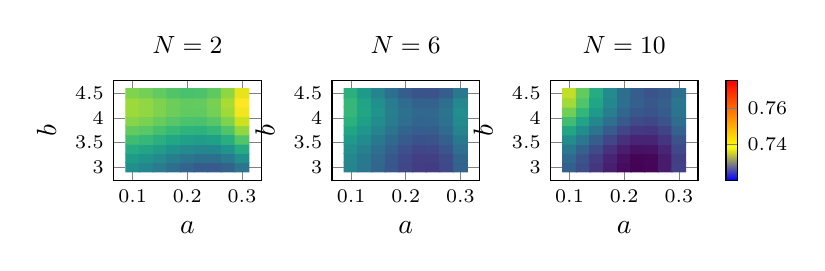
\begin{tikzpicture}
\begin{groupplot}[group style={group size=3 by 1,horizontal sep=0.9cm},width=0.285\textwidth,height=0.235\textwidth,view={0}{90},xlabel={$a$},ylabel={$b$},xtick={0.10,0.20,0.30},ytick={3.0,3.5,4.0,4.5},tick label style={font=\scriptsize},title style={font=\small\bfseries}]
\nextgroupplot[title={$N=2$},point meta min=0.72022885,point meta max=0.77569756]
\addplot[matrix plot*,mesh/cols=9,point meta=explicit,colormap/viridis] coordinates {(0.10000,3.00000) [0.74764669] (0.12500,3.00000) [0.74593625] (0.15000,3.00000) [0.74335840] (0.17500,3.00000) [0.74048873] (0.20000,3.00000) [0.73790280] (0.22500,3.00000) [0.73617619] (0.25000,3.00000) [0.73588447] (0.27500,3.00000) [0.73760323] (0.30000,3.00000) [0.74190803] (0.10000,3.18750) [0.75042771] (0.12500,3.18750) [0.74893964] (0.15000,3.18750) [0.74662778] (0.17500,3.18750) [0.74406770] (0.20000,3.18750) [0.74183499] (0.22500,3.18750) [0.74050522] (0.25000,3.18750) [0.74065396] (0.27500,3.18750) [0.74285679] (0.30000,3.18750) [0.74768928] (0.10000,3.37500) [0.75420146] (0.12500,3.37500) [0.75289316] (0.15000,3.37500) [0.75080469] (0.17500,3.37500) [0.74851162] (0.20000,3.37500) [0.74658954] (0.22500,3.37500) [0.74561401] (0.25000,3.37500) [0.74616061] (0.27500,3.37500) [0.74880492] (0.30000,3.37500) [0.75412251] (0.10000,3.56250) [0.75838524] (0.12500,3.56250) [0.75721412] (0.15000,3.56250) [0.75530645] (0.17500,3.56250) [0.75323780] (0.20000,3.56250) [0.75158375] (0.22500,3.56250) [0.75091987] (0.25000,3.56250) [0.75182174] (0.27500,3.56250) [0.75486494] (0.30000,3.56250) [0.76062504] (0.10000,3.75000) [0.76239638] (0.12500,3.75000) [0.76131985] (0.15000,3.75000) [0.75955038] (0.17500,3.75000) [0.75766356] (0.20000,3.75000) [0.75623494] (0.22500,3.75000) [0.75584013] (0.25000,3.75000) [0.75705467] (0.27500,3.75000) [0.76045417] (0.30000,3.75000) [0.76661418] (0.10000,3.93750) [0.76565221] (0.12500,3.93750) [0.76462767] (0.15000,3.93750) [0.76295381] (0.17500,3.93750) [0.76120621] (0.20000,3.93750) [0.75996045] (0.22500,3.93750) [0.75979210] (0.25000,3.93750) [0.76127673] (0.27500,3.93750) [0.76498992] (0.30000,3.93750) [0.77150725] (0.10000,4.12500) [0.76757003] (0.12500,4.12500) [0.76655489] (0.15000,4.12500) [0.76493405] (0.17500,4.12500) [0.76328309] (0.20000,4.12500) [0.76217758] (0.22500,4.12500) [0.76219310] (0.25000,4.12500) [0.76390522] (0.27500,4.12500) [0.76788952] (0.30000,4.12500) [0.77472158] (0.10000,4.31250) [0.76756716] (0.12500,4.31250) [0.76651883] (0.15000,4.31250) [0.76490842] (0.17500,4.31250) [0.76331150] (0.20000,4.31250) [0.76230365] (0.22500,4.31250) [0.76246045] (0.25000,4.31250) [0.76435747] (0.27500,4.31250) [0.76857029] (0.30000,4.31250) [0.77567448] (0.10000,4.50000) [0.76506093] (0.12500,4.50000) [0.76393681] (0.15000,4.50000) [0.76229423] (0.17500,4.50000) [0.76070876] (0.20000,4.50000) [0.75975599] (0.22500,4.50000) [0.76001147] (0.25000,4.50000) [0.76205080] (0.27500,4.50000) [0.76644954] (0.30000,4.50000) [0.77378327]};
\nextgroupplot[title={$N=6$},point meta min=0.72022885,point meta max=0.77569756]
\addplot[matrix plot*,mesh/cols=9,point meta=explicit,colormap/viridis] coordinates {(0.10000,3.00000) [0.74548483] (0.12500,3.00000) [0.74235133] (0.15000,3.00000) [0.73866979] (0.17500,3.00000) [0.73501579] (0.20000,3.00000) [0.73196491] (0.22500,3.00000) [0.73009271] (0.25000,3.00000) [0.72997478] (0.27500,3.00000) [0.73218669] (0.30000,3.00000) [0.73730401] (0.10000,3.18750) [0.74579368] (0.12500,3.18750) [0.74258291] (0.15000,3.18750) [0.73886772] (0.17500,3.18750) [0.73522368] (0.20000,3.18750) [0.73222637] (0.22500,3.18750) [0.73045137] (0.25000,3.18750) [0.73047425] (0.27500,3.18750) [0.73287059] (0.30000,3.18750) [0.73821597] (0.10000,3.37500) [0.74752958] (0.12500,3.37500) [0.74419894] (0.15000,3.37500) [0.74040750] (0.17500,3.37500) [0.73673083] (0.20000,3.37500) [0.73374450] (0.22500,3.37500) [0.73202411] (0.25000,3.37500) [0.73214521] (0.27500,3.37500) [0.73468339] (0.30000,3.37500) [0.74021423] (0.10000,3.56250) [0.75010984] (0.12500,3.56250) [0.74661674] (0.15000,3.56250) [0.74270645] (0.17500,3.56250) [0.73895456] (0.20000,3.56250) [0.73593663] (0.22500,3.56250) [0.73422824] (0.25000,3.56250) [0.73440498] (0.27500,3.56250) [0.73704241] (0.30000,3.56250) [0.74271610] (0.10000,3.75000) [0.75295179] (0.12500,3.75000) [0.74925363] (0.15000,3.75000) [0.74518191] (0.17500,3.75000) [0.74131219] (0.20000,3.75000) [0.73822007] (0.22500,3.75000) [0.73648110] (0.25000,3.75000) [0.73667087] (0.27500,3.75000) [0.73936495] (0.30000,3.75000) [0.74513892] (0.10000,3.93750) [0.75547274] (0.12500,3.93750) [0.75152693] (0.15000,3.93750) [0.74725118] (0.17500,3.93750) [0.74322105] (0.20000,3.93750) [0.74001213] (0.22500,3.93750) [0.73819999] (0.25000,3.93750) [0.73836020] (0.27500,3.93750) [0.74106834] (0.30000,3.93750) [0.74689999] (0.10000,4.12500) [0.75709000] (0.12500,4.12500) [0.75285396] (0.15000,4.12500) [0.74833158] (0.17500,4.12500) [0.74409845] (0.20000,4.12500) [0.74073014] (0.22500,4.12500) [0.73880223] (0.25000,4.12500) [0.73889029] (0.27500,4.12500) [0.74156991] (0.30000,4.12500) [0.74741664] (0.10000,4.31250) [0.75722091] (0.12500,4.31250) [0.75265203] (0.15000,4.31250) [0.74784044] (0.17500,4.31250) [0.74336171] (0.20000,4.31250) [0.73979142] (0.22500,4.31250) [0.73770515] (0.25000,4.31250) [0.73767847] (0.27500,4.31250) [0.74028696] (0.30000,4.31250) [0.74610619] (0.10000,4.50000) [0.75528277] (0.12500,4.50000) [0.75033847] (0.15000,4.50000) [0.74519507] (0.17500,4.50000) [0.74042815] (0.20000,4.50000) [0.73661329] (0.22500,4.50000) [0.73432607] (0.25000,4.50000) [0.73414205] (0.27500,4.50000) [0.73663682] (0.30000,4.50000) [0.74238594]};
\nextgroupplot[title={$N=10$},point meta min=0.72022885,point meta max=0.77569756,colorbar,colorbar style={width=1.5mm,yticklabel style={font=\scriptsize}}]
\addplot[matrix plot*,mesh/cols=9,point meta=explicit,colormap/viridis] coordinates {(0.10000,3.00000) [0.73710573] (0.12500,3.00000) [0.73307731] (0.15000,3.00000) [0.72882022] (0.17500,3.00000) [0.72491004] (0.20000,3.00000) [0.72192234] (0.22500,3.00000) [0.72043270] (0.25000,3.00000) [0.72101670] (0.27500,3.00000) [0.72424990] (0.30000,3.00000) [0.73070789] (0.10000,3.18750) [0.73885245] (0.12500,3.18750) [0.73444711] (0.15000,3.18750) [0.72985673] (0.17500,3.18750) [0.72565687] (0.20000,3.18750) [0.72242311] (0.22500,3.18750) [0.72073102] (0.25000,3.18750) [0.72115619] (0.27500,3.18750) [0.72427419] (0.30000,3.18750) [0.73066058] (0.10000,3.37500) [0.74246053] (0.12500,3.37500) [0.73763569] (0.15000,3.37500) [0.73266942] (0.17500,3.37500) [0.72813728] (0.20000,3.37500) [0.72461487] (0.22500,3.37500) [0.72267775] (0.25000,3.37500) [0.72290149] (0.27500,3.37500) [0.72586169] (0.30000,3.37500) [0.73213391] (0.10000,3.56250) [0.74734731] (0.12500,3.56250) [0.74206036] (0.15000,3.56250) [0.73667560] (0.17500,3.56250) [0.73176860] (0.20000,3.56250) [0.72791494] (0.22500,3.56250) [0.72569019] (0.25000,3.56250) [0.72566993] (0.27500,3.56250) [0.72842973] (0.30000,3.56250) [0.73454517] (0.10000,3.75000) [0.75293009] (0.12500,3.75000) [0.74713845] (0.15000,3.75000) [0.74129261] (0.17500,3.75000) [0.73596815] (0.20000,3.75000) [0.73174065] (0.22500,3.75000) [0.72918567] (0.25000,3.75000) [0.72887881] (0.27500,3.75000) [0.73139562] (0.30000,3.75000) [0.73731169] (0.10000,3.93750) [0.75862619] (0.12500,3.93750) [0.75228726] (0.15000,3.93750) [0.74593776] (0.17500,3.93750) [0.74015325] (0.20000,3.93750) [0.73550931] (0.22500,3.93750) [0.73258152] (0.25000,3.93750) [0.73194545] (0.27500,3.93750) [0.73417669] (0.30000,3.93750) [0.73985080] (0.10000,4.12500) [0.76385294] (0.12500,4.12500) [0.75692413] (0.15000,4.12500) [0.75002836] (0.17500,4.12500) [0.74374121] (0.20000,4.12500) [0.73863824] (0.22500,4.12500) [0.73529504] (0.25000,4.12500) [0.73428719] (0.27500,4.12500) [0.73619025] (0.30000,4.12500) [0.74157980] (0.10000,4.31250) [0.76802765] (0.12500,4.31250) [0.76046637] (0.15000,4.31250) [0.75298174] (0.17500,4.31250) [0.74614935] (0.20000,4.31250) [0.74054476] (0.22500,4.31250) [0.73674356] (0.25000,4.31250) [0.73532132] (0.27500,4.31250) [0.73685362] (0.30000,4.31250) [0.74191603] (0.10000,4.50000) [0.77056764] (0.12500,4.50000) [0.76233129] (0.15000,4.50000) [0.75421522] (0.17500,4.50000) [0.74679500] (0.20000,4.50000) [0.74064620] (0.22500,4.50000) [0.73634440] (0.25000,4.50000) [0.73446519] (0.27500,4.50000) [0.73558412] (0.30000,4.50000) [0.74027679]};
\end{groupplot}
\end{tikzpicture}
\vspace{-0.25em}
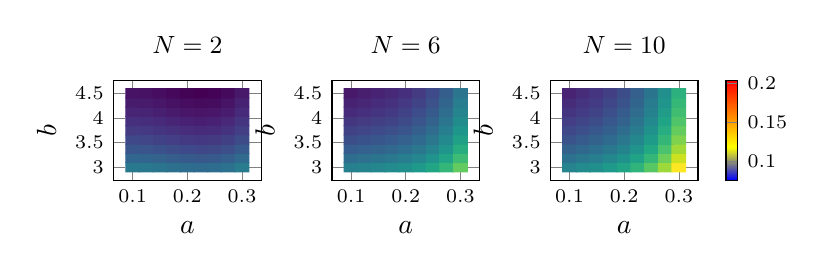
\begin{tikzpicture}
\begin{groupplot}[group style={group size=3 by 1,horizontal sep=0.9cm},width=0.285\textwidth,height=0.235\textwidth,view={0}{90},xlabel={$a$},ylabel={$b$},xtick={0.10,0.20,0.30},ytick={3.0,3.5,4.0,4.5},tick label style={font=\scriptsize},title style={font=\small\bfseries}]
\nextgroupplot[title={$N=2$},point meta min=0.07604129,point meta max=0.20396690]
\addplot[matrix plot*,mesh/cols=9,point meta=explicit,colormap/viridis] coordinates {(0.10000,3.00000) [0.12781977] (0.12500,3.00000) [0.12694741] (0.15000,3.00000) [0.12519697] (0.17500,3.00000) [0.12315513] (0.20000,3.00000) [0.12140857] (0.22500,3.00000) [0.12054396] (0.25000,3.00000) [0.12114799] (0.27500,3.00000) [0.12380734] (0.30000,3.00000) [0.12910868] (0.10000,3.18750) [0.11815646] (0.12500,3.18750) [0.11735190] (0.15000,3.18750) [0.11565792] (0.17500,3.18750) [0.11366121] (0.20000,3.18750) [0.11194844] (0.22500,3.18750) [0.11110629] (0.25000,3.18750) [0.11172145] (0.27500,3.18750) [0.11438058] (0.30000,3.18750) [0.11967037] (0.10000,3.37500) [0.11009691] (0.12500,3.37500) [0.10935613] (0.15000,3.37500) [0.10771459] (0.17500,3.37500) [0.10575898] (0.20000,3.37500) [0.10407597] (0.22500,3.37500) [0.10325225] (0.25000,3.37500) [0.10387450] (0.27500,3.37500) [0.10652939] (0.30000,3.37500) [0.11180360] (0.10000,3.56250) [0.10340311] (0.12500,3.56250) [0.10272206] (0.15000,3.56250) [0.10112894] (0.17500,3.56250) [0.09921040] (0.20000,3.56250) [0.09755314] (0.22500,3.56250) [0.09674382] (0.25000,3.56250) [0.09736913] (0.27500,3.56250) [0.10001575] (0.30000,3.56250) [0.10527036] (0.10000,3.75000) [0.09783702] (0.12500,3.75000) [0.09721169] (0.15000,3.75000) [0.09566295] (0.17500,3.75000) [0.09377746] (0.20000,3.75000) [0.09214191] (0.22500,3.75000) [0.09134297] (0.25000,3.75000) [0.09196732] (0.27500,3.75000) [0.09460165] (0.30000,3.75000) [0.09983262] (0.10000,3.93750) [0.09316062] (0.12500,3.93750) [0.09258699] (0.15000,3.93750) [0.09107860] (0.17500,3.93750) [0.08922214] (0.20000,3.93750) [0.08760427] (0.22500,3.93750) [0.08681168] (0.25000,3.93750) [0.08743104] (0.27500,3.93750) [0.09004905] (0.30000,3.93750) [0.09525236] (0.10000,4.12500) [0.08913590] (0.12500,4.12500) [0.08860994] (0.15000,4.12500) [0.08713788] (0.17500,4.12500) [0.08530640] (0.20000,4.12500) [0.08370219] (0.22500,4.12500) [0.08291193] (0.25000,4.12500) [0.08352228] (0.27500,4.12500) [0.08611993] (0.30000,4.12500) [0.09129156] (0.10000,4.31250) [0.08552483] (0.12500,4.31250) [0.08504250] (0.15000,4.31250) [0.08360275] (0.17500,4.31250) [0.08179224] (0.20000,4.31250) [0.08019766] (0.22500,4.31250) [0.07940569] (0.25000,4.31250) [0.08000300] (0.27500,4.31250) [0.08257628] (0.30000,4.31250) [0.08771220] (0.10000,4.50000) [0.08208939] (0.12500,4.50000) [0.08164667] (0.15000,4.50000) [0.08023520] (0.17500,4.50000) [0.07844163] (0.20000,4.50000) [0.07685266] (0.22500,4.50000) [0.07605495] (0.25000,4.50000) [0.07663520] (0.27500,4.50000) [0.07918007] (0.30000,4.50000) [0.08427625]};
\nextgroupplot[title={$N=6$},point meta min=0.07604129,point meta max=0.20396690]
\addplot[matrix plot*,mesh/cols=9,point meta=explicit,colormap/viridis] coordinates {(0.10000,3.00000) [0.13141377] (0.12500,3.00000) [0.13327680] (0.15000,3.00000) [0.13493932] (0.17500,3.00000) [0.13698801] (0.20000,3.00000) [0.14000956] (0.22500,3.00000) [0.14459063] (0.25000,3.00000) [0.15131792] (0.27500,3.00000) [0.16077809] (0.30000,3.00000) [0.17355782] (0.10000,3.18750) [0.12150982] (0.12500,3.18750) [0.12342470] (0.15000,3.18750) [0.12512774] (0.17500,3.18750) [0.12720562] (0.20000,3.18750) [0.13024501] (0.22500,3.18750) [0.13483259] (0.25000,3.18750) [0.14155505] (0.27500,3.18750) [0.15099905] (0.30000,3.18750) [0.16375129] (0.10000,3.37500) [0.11322649] (0.12500,3.37500) [0.11518920] (0.15000,3.37500) [0.11692873] (0.17500,3.37500) [0.11903176] (0.20000,3.37500) [0.12208497] (0.22500,3.37500) [0.12667503] (0.25000,3.37500) [0.13338863] (0.27500,3.37500) [0.14281245] (0.30000,3.37500) [0.15553316] (0.10000,3.56250) [0.10632576] (0.12500,3.56250) [0.10833227] (0.15000,3.56250) [0.11010426] (0.17500,3.56250) [0.11222842] (0.20000,3.56250) [0.11529142] (0.22500,3.56250) [0.11987994] (0.25000,3.56250) [0.12658066] (0.27500,3.56250) [0.13598026] (0.30000,3.56250) [0.14866542] (0.10000,3.75000) [0.10056961] (0.12500,3.75000) [0.10261589] (0.15000,3.75000) [0.10441632] (0.17500,3.75000) [0.10655757] (0.20000,3.75000) [0.10962634] (0.22500,3.75000) [0.11420928] (0.25000,3.75000) [0.12089310] (0.27500,3.75000) [0.13026446] (0.30000,3.75000) [0.14291003] (0.10000,3.93750) [0.09572001] (0.12500,3.93750) [0.09780203] (0.15000,3.93750) [0.09962687] (0.17500,3.93750) [0.10178120] (0.20000,3.93750) [0.10485170] (0.22500,3.93750) [0.10942505] (0.25000,3.93750) [0.11608793] (0.27500,3.93750) [0.12542702] (0.30000,3.93750) [0.13802899] (0.10000,4.12500) [0.09153894] (0.12500,4.12500) [0.09365269] (0.15000,4.12500) [0.09549790] (0.17500,4.12500) [0.09766128] (0.20000,4.12500) [0.10072949] (0.22500,4.12500) [0.10528922] (0.25000,4.12500) [0.11192713] (0.27500,4.12500) [0.12122992] (0.30000,4.12500) [0.13378427] (0.10000,4.31250) [0.08778839] (0.12500,4.31250) [0.08992982] (0.15000,4.31250) [0.09179139] (0.17500,4.31250) [0.09395979] (0.20000,4.31250) [0.09702168] (0.22500,4.31250) [0.10156376] (0.25000,4.31250) [0.10817269] (0.27500,4.31250) [0.11743515] (0.30000,4.31250) [0.12993783] (0.10000,4.50000) [0.08423032] (0.12500,4.50000) [0.08639541] (0.15000,4.50000) [0.08826932] (0.17500,4.50000) [0.09043870] (0.20000,4.50000) [0.09349026] (0.22500,4.50000) [0.09801065] (0.25000,4.50000) [0.10458657] (0.27500,4.50000) [0.11380468] (0.30000,4.50000) [0.12625168]};
\nextgroupplot[title={$N=10$},point meta min=0.07604129,point meta max=0.20396690,colorbar,colorbar style={width=1.5mm,yticklabel style={font=\scriptsize}}]
\addplot[matrix plot*,mesh/cols=9,point meta=explicit,colormap/viridis] coordinates {(0.10000,3.00000) [0.13365965] (0.12500,3.00000) [0.13667158] (0.15000,3.00000) [0.14016057] (0.17500,3.00000) [0.14471331] (0.20000,3.00000) [0.15091647] (0.22500,3.00000) [0.15935673] (0.25000,3.00000) [0.17062077] (0.27500,3.00000) [0.18529526] (0.30000,3.00000) [0.20396690] (0.10000,3.18750) [0.12394512] (0.12500,3.18750) [0.12699295] (0.15000,3.18750) [0.13050652] (0.17500,3.18750) [0.13507249] (0.20000,3.18750) [0.14127754] (0.22500,3.18750) [0.14970836] (0.25000,3.18750) [0.16095163] (0.27500,3.18750) [0.17559402] (0.30000,3.18750) [0.19422221] (0.10000,3.37500) [0.11586807] (0.12500,3.37500) [0.11894779] (0.15000,3.37500) [0.12248189] (0.17500,3.37500) [0.12705707] (0.20000,3.37500) [0.13325999] (0.22500,3.37500) [0.14167735] (0.25000,3.37500) [0.15289581] (0.27500,3.37500) [0.16750206] (0.30000,3.37500) [0.18608278] (0.10000,3.56250) [0.10919048] (0.12500,3.56250) [0.11229805] (0.15000,3.56250) [0.11584867] (0.17500,3.56250) [0.12042902] (0.20000,3.56250) [0.12662579] (0.22500,3.56250) [0.13502565] (0.25000,3.56250) [0.14621529] (0.27500,3.56250) [0.16078138] (0.30000,3.56250) [0.17931059] (0.10000,3.75000) [0.10367433] (0.12500,3.75000) [0.10680571] (0.15000,3.75000) [0.11036882] (0.17500,3.75000) [0.11495033] (0.20000,3.75000) [0.12113692] (0.22500,3.75000) [0.12951526] (0.25000,3.75000) [0.14067204] (0.27500,3.75000) [0.15519394] (0.30000,3.75000) [0.17366763] (0.10000,3.93750) [0.09908158] (0.12500,3.93750) [0.10223277] (0.15000,3.93750) [0.10580434] (0.17500,3.93750) [0.11038297] (0.20000,3.93750) [0.11655535] (0.22500,3.93750) [0.12490814] (0.25000,3.93750) [0.13602804] (0.27500,3.93750) [0.15050172] (0.30000,3.93750) [0.16891586] (0.10000,4.12500) [0.09517423] (0.12500,4.12500) [0.09834118] (0.15000,4.12500) [0.10191719] (0.17500,4.12500) [0.10648892] (0.20000,4.12500) [0.11264306] (0.22500,4.12500) [0.12096629] (0.25000,4.12500) [0.13204528] (0.27500,4.12500) [0.14646671] (0.30000,4.12500) [0.16481727] (0.10000,4.31250) [0.09171425] (0.12500,4.31250) [0.09489294] (0.15000,4.31250) [0.09846936] (0.17500,4.31250) [0.10303016] (0.20000,4.31250) [0.10916203] (0.22500,4.31250) [0.11745166] (0.25000,4.31250) [0.12848572] (0.27500,4.31250) [0.14285088] (0.30000,4.31250) [0.16113383] (0.10000,4.50000) [0.08846361] (0.12500,4.50000) [0.09165002] (0.15000,4.50000) [0.09522282] (0.17500,4.50000) [0.09976866] (0.20000,4.50000) [0.10587425] (0.22500,4.50000) [0.11412625] (0.25000,4.50000) [0.12511134] (0.27500,4.50000) [0.13941620] (0.30000,4.50000) [0.15762752]};
\end{groupplot}
\end{tikzpicture}
\vspace{-0.25em}
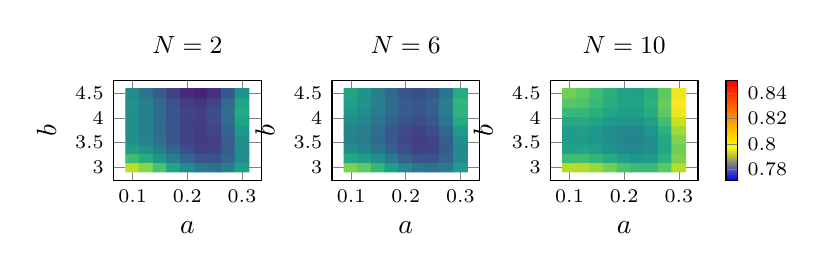
\begin{tikzpicture}
\begin{groupplot}[group style={group size=3 by 1,horizontal sep=0.9cm},width=0.285\textwidth,height=0.235\textwidth,view={0}{90},xlabel={$a$},ylabel={$b$},xtick={0.10,0.20,0.30},ytick={3.0,3.5,4.0,4.5},tick label style={font=\scriptsize},title style={font=\small\bfseries}]
\nextgroupplot[title={$N=2$},point meta min=0.77178663,point meta max=0.84979756]
\addplot[matrix plot*,mesh/cols=9,point meta=explicit,colormap/viridis] coordinates {(0.10000,3.00000) [0.84178395] (0.12500,3.00000) [0.83579463] (0.15000,3.00000) [0.82730396] (0.17500,3.00000) [0.81795210] (0.20000,3.00000) [0.80937922] (0.22500,3.00000) [0.80322547] (0.25000,3.00000) [0.80113104] (0.27500,3.00000) [0.80473608] (0.30000,3.00000) [0.81568076] (0.10000,3.18750) [0.82552402] (0.12500,3.18750) [0.82032406] (0.15000,3.18750) [0.81277906] (0.17500,3.18750) [0.80452918] (0.20000,3.18750) [0.79721459] (0.22500,3.18750) [0.79247545] (0.25000,3.18750) [0.79195193] (0.27500,3.18750) [0.79728420] (0.30000,3.18750) [0.81011242] (0.10000,3.37500) [0.81563648] (0.12500,3.37500) [0.81097122] (0.15000,3.37500) [0.80411723] (0.17500,3.37500) [0.79671468] (0.20000,3.37500) [0.79040373] (0.22500,3.37500) [0.78682454] (0.25000,3.37500) [0.78761729] (0.27500,3.37500) [0.79442214] (0.30000,3.37500) [0.80887925] (0.10000,3.56250) [0.81067558] (0.12500,3.56250) [0.80629037] (0.15000,3.56250) [0.79987275] (0.17500,3.56250) [0.79306287] (0.20000,3.56250) [0.78750090] (0.22500,3.56250) [0.78482702] (0.25000,3.56250) [0.78668138] (0.27500,3.56250) [0.79470415] (0.30000,3.56250) [0.81053550] (0.10000,3.75000) [0.80919559] (0.12500,3.75000) [0.80483578] (0.15000,3.75000) [0.79859986] (0.17500,3.75000) [0.79212800] (0.20000,3.75000) [0.78706037] (0.22500,3.75000) [0.78503713] (0.25000,3.75000) [0.78769845] (0.27500,3.75000) [0.79668449] (0.30000,3.75000) [0.81363543] (0.10000,3.93750) [0.80975076] (0.12500,3.93750) [0.80516169] (0.15000,3.93750) [0.79885283] (0.17500,3.93750) [0.79246434] (0.20000,3.93750) [0.78763639] (0.22500,3.93750) [0.78600915] (0.25000,3.93750) [0.78922277] (0.27500,3.93750) [0.79891743] (0.30000,3.93750) [0.81673330] (0.10000,4.12500) [0.81089536] (0.12500,4.12500) [0.80582238] (0.15000,4.12500) [0.79918592] (0.17500,4.12500) [0.79262614] (0.20000,4.12500) [0.78778322] (0.22500,4.12500) [0.78629732] (0.25000,4.12500) [0.78980859] (0.27500,4.12500) [0.79995722] (0.30000,4.12500) [0.81838336] (0.10000,4.31250) [0.81118364] (0.12500,4.31250) [0.80537209] (0.15000,4.31250) [0.79815338] (0.17500,4.31250) [0.79116767] (0.20000,4.31250) [0.78605512] (0.22500,4.31250) [0.78445591] (0.25000,4.31250) [0.78801018] (0.27500,4.31250) [0.79835812] (0.30000,4.31250) [0.81713989] (0.10000,4.50000) [0.80916986] (0.12500,4.50000) [0.80236510] (0.15000,4.50000) [0.79430949] (0.17500,4.50000) [0.78664318] (0.20000,4.50000) [0.78100636] (0.22500,4.50000) [0.77903917] (0.25000,4.50000) [0.78238180] (0.27500,4.50000) [0.79267440] (0.30000,4.50000) [0.81155714]};
\nextgroupplot[title={$N=6$},point meta min=0.77178663,point meta max=0.84979756]
\addplot[matrix plot*,mesh/cols=9,point meta=explicit,colormap/viridis] coordinates {(0.10000,3.00000) [0.83425712] (0.12500,3.00000) [0.83037940] (0.15000,3.00000) [0.82362981] (0.17500,3.00000) [0.81564853] (0.20000,3.00000) [0.80807572] (0.22500,3.00000) [0.80255155] (0.25000,3.00000) [0.80071618] (0.27500,3.00000) [0.80420978] (0.30000,3.00000) [0.81467252] (0.10000,3.18750) [0.81873657] (0.12500,3.18750) [0.81554254] (0.15000,3.18750) [0.80963295] (0.17500,3.18750) [0.80264798] (0.20000,3.18750) [0.79622779] (0.22500,3.18750) [0.79201256] (0.25000,3.18750) [0.79164244] (0.27500,3.18750) [0.79675760] (0.30000,3.18750) [0.80899821] (0.10000,3.37500) [0.80995061] (0.12500,3.37500) [0.80718561] (0.15000,3.37500) [0.80186136] (0.17500,3.37500) [0.79561805] (0.20000,3.37500) [0.79009584] (0.22500,3.37500) [0.78693488] (0.25000,3.37500) [0.78777536] (0.27500,3.37500) [0.79425743] (0.30000,3.37500) [0.80802126] (0.10000,3.56250) [0.80645349] (0.12500,3.56250) [0.80386287] (0.15000,3.56250) [0.79886932] (0.17500,3.56250) [0.79311301] (0.20000,3.56250) [0.78823411] (0.22500,3.56250) [0.78587279] (0.25000,3.56250) [0.78766921] (0.27500,3.56250) [0.79526353] (0.30000,3.56250) [0.81029593] (0.10000,3.75000) [0.80679948] (0.12500,3.75000) [0.80412858] (0.15000,3.75000) [0.79921107] (0.17500,3.75000) [0.79368711] (0.20000,3.75000) [0.78919688] (0.22500,3.75000) [0.78738054] (0.25000,3.75000) [0.78987824] (0.27500,3.75000) [0.79833017] (0.30000,3.75000) [0.81437648] (0.10000,3.93750) [0.80954283] (0.12500,3.93750) [0.80653700] (0.15000,3.93750) [0.80144088] (0.17500,3.93750) [0.79589462] (0.20000,3.93750) [0.79153840] (0.22500,3.93750) [0.79001238] (0.25000,3.93750) [0.79295673] (0.27500,3.93750) [0.80201160] (0.30000,3.93750) [0.81881717] (0.10000,4.12500) [0.81323780] (0.12500,4.12500) [0.80964240] (0.15000,4.12500) [0.80411301] (0.17500,4.12500) [0.79828980] (0.20000,4.12500) [0.79381293] (0.22500,4.12500) [0.79232258] (0.25000,4.12500) [0.79545891] (0.27500,4.12500) [0.80486208] (0.30000,4.12500) [0.82217227] (0.10000,4.31250) [0.81643866] (0.12500,4.31250) [0.81199902] (0.15000,4.31250) [0.80578171] (0.17500,4.31250) [0.79942689] (0.20000,4.31250) [0.79457474] (0.22500,4.31250) [0.79286541] (0.25000,4.31250) [0.79593906] (0.27500,4.31250) [0.80543588] (0.30000,4.31250) [0.82299602] (0.10000,4.50000) [0.81769966] (0.12500,4.50000) [0.81216114] (0.15000,4.50000) [0.80500125] (0.17500,4.50000) [0.79786018] (0.20000,4.50000) [0.79237807] (0.22500,4.50000) [0.79019510] (0.25000,4.50000) [0.79295144] (0.27500,4.50000) [0.80228725] (0.30000,4.50000) [0.81984269]};
\nextgroupplot[title={$N=10$},point meta min=0.77178663,point meta max=0.84979756,colorbar,colorbar style={width=1.5mm,yticklabel style={font=\scriptsize}}]
\addplot[matrix plot*,mesh/cols=9,point meta=explicit,colormap/viridis] coordinates {(0.10000,3.00000) [0.84112887] (0.12500,3.00000) [0.84100578] (0.15000,3.00000) [0.83764033] (0.17500,3.00000) [0.83267268] (0.20000,3.00000) [0.82774300] (0.22500,3.00000) [0.82449144] (0.25000,3.00000) [0.82455819] (0.27500,3.00000) [0.82958340] (0.30000,3.00000) [0.84120723] (0.10000,3.18750) [0.82540239] (0.12500,3.18750) [0.82585732] (0.15000,3.18750) [0.82322620] (0.17500,3.18750) [0.81914919] (0.20000,3.18750) [0.81526646] (0.22500,3.18750) [0.81321817] (0.25000,3.18750) [0.81464450] (0.27500,3.18750) [0.82118560] (0.30000,3.18750) [0.83448164] (0.10000,3.37500) [0.81677270] (0.12500,3.37500) [0.81755099] (0.15000,3.37500) [0.81539955] (0.17500,3.37500) [0.81195853] (0.20000,3.37500) [0.80886810] (0.22500,3.37500) [0.80776842] (0.25000,3.37500) [0.81029968] (0.27500,3.37500) [0.81810202] (0.30000,3.37500) [0.83281561] (0.10000,3.56250) [0.81379405] (0.12500,3.56250) [0.81464105] (0.15000,3.56250) [0.81271463] (0.17500,3.56250) [0.80965495] (0.20000,3.56250) [0.80710217] (0.22500,3.56250) [0.80669645] (0.25000,3.56250) [0.81007798] (0.27500,3.56250) [0.81888691] (0.30000,3.56250) [0.83476340] (0.10000,3.75000) [0.81502071] (0.12500,3.75000) [0.81568177] (0.15000,3.75000) [0.81372571] (0.17500,3.75000) [0.81079271] (0.20000,3.75000) [0.80852293] (0.22500,3.75000) [0.80855652] (0.25000,3.75000) [0.81253367] (0.27500,3.75000) [0.82209453] (0.30000,3.75000) [0.83887927] (0.10000,3.93750) [0.81900693] (0.12500,3.93750) [0.81922739] (0.15000,3.93750) [0.81698706] (0.17500,3.93750) [0.81392608] (0.20000,3.93750) [0.81168464] (0.22500,3.93750) [0.81190289] (0.25000,3.93750) [0.81622101] (0.27500,3.93750) [0.82627915] (0.30000,3.93750) [0.84371748] (0.10000,4.12500) [0.82430697] (0.12500,4.12500) [0.82383219] (0.15000,4.12500) [0.82105292] (0.17500,4.12500) [0.81760932] (0.20000,4.12500) [0.81514157] (0.22500,4.12500) [0.81528982] (0.25000,4.12500) [0.81969425] (0.27500,4.12500) [0.82999501] (0.30000,4.12500) [0.84783229] (0.10000,4.31250) [0.82947510] (0.12500,4.31250) [0.82805041] (0.15000,4.31250) [0.82447755] (0.17500,4.31250) [0.82039668] (0.20000,4.31250) [0.81744796] (0.22500,4.31250) [0.81727157] (0.25000,4.31250) [0.82150765] (0.27500,4.31250) [0.83179640] (0.30000,4.31250) [0.84977795] (0.10000,4.50000) [0.83306557] (0.12500,4.50000) [0.83043633] (0.15000,4.50000) [0.82581523] (0.17500,4.50000) [0.82084242] (0.20000,4.50000) [0.81715809] (0.22500,4.50000) [0.81640239] (0.25000,4.50000) [0.82021549] (0.27500,4.50000) [0.83023755] (0.30000,4.50000) [0.84810874]};
\end{groupplot}
\end{tikzpicture}
\caption{三次Ridge在$N=2,6,10$下的九组$(a,b)$合法切片：第一行为$R$，第二行为$P$，第三行为$U$。同一响应的颜色范围固定。}\label{fig:surface}
\end{figure}

在$81\times81\times5$个合法网格点上，三项预测均未超出样本极差加5\%容差，且$P$关于$b$保持全域单调下降，未发现虚假尖峰或异常极值。

\subsection{外推边界}
\begin{table}[H]\centering\small
\caption{留一水平压力测试的最差NRMSE汇总}\label{tab:boundary}
\begin{tabular}{lrrr}
\toprule
测试类型 & 最大$R$-NRMSE & 最大$P$-NRMSE & 最大$U$-NRMSE \\
\midrule
内部水平插值 & 0.0881 & 0.0445 & 0.1195 \\
边界水平外推 & 2.0595 & 0.3965 & 2.1200 \\
\bottomrule
\end{tabular}
\end{table}

内部水平留出的误差显著低于边界外推误差，但$U$对未见水平仍较敏感；留出$a=0.30$后$R,U$的外推误差显著放大。因此，当前代理模型适用于全部80点共同覆盖的设计域内插值，但不能用于$a>0.30$、$b>4.5$等无数据区域。

\section{最终代理模型及问题3接口}
令$\bm\phi_3(\bm\xi)$按附录的19项顺序展开，并以特征均值$m_q$和尺度$t_q$二次标准化，最终模型统一为
\[
\widehat y_k=\beta_{0k}+\sum_{q=1}^{19}\beta_{qk}\frac{\phi_q(\bm\xi)-m_q}{t_q},\qquad k\in\{R,P,U\}.
\]
为使显式模型可复现，原始输入的标准化参数、截距与岭参数汇总于表\ref{tab:reproduce}；完整非截距系数与特征二次标准化参数见附录。
\begin{table}[H]\centering\small
\caption{最终代理模型的复现参数}\label{tab:reproduce}
\begin{tabular}{cccc}
\toprule
参数 & $R$ & $P$ & $U$ \\
\midrule
截距 $\beta_{0k}$ & 0.746101800 & 0.1170519125 & 0.8131816625 \\
岭参数 $\lambda_k$ & $10^{-5}$ & $10^{-2}$ & $10^{-3}$ \\
\bottomrule
\end{tabular}\\[3pt]
$\bm\mu_x=(0.1875,\ 3.75,\ 6)^{\mathrm T}$，\quad
$\bm s_x=(0.073951,\ 0.559017,\ 2.828427)^{\mathrm T}$。
\end{table}
无针肋支路为
\[
\widehat y_{k,0}(b)=\operatorname{PCHIP}\{(b_i,y_{ki})\}_{i=1}^{4},\qquad 3\le b\le4.5.
\]
问题3可直接求解
\[
\begin{gathered}
\min\left(\widehat R(a,b,N),\widehat P(a,b,N),\widehat U(a,b,N)\right),\\
0.10\le a\le0.30,\quad3\le b\le4.5,\quad N\in\{2,4,6,8,10\}.
\end{gathered}
\]
综上，三次Ridge在重复折外验证、数值稳定性和合法曲面检验中均表现最佳或处于重复交叉验证波动的等价带内，三个响应的OOF-NRMSE均低于0.005。它可可靠刻画附件覆盖域内的非线性及交互映射，并直接供问题3多目标优化调用；无针肋结构采用独立PCHIP支路，模型不在两类结构间插值，也不承担设计域外预测。

\appendix
\section{无针肋支路PCHIP节点}
\begin{table}[H]\centering\small
\caption{无针肋结构的PCHIP插值节点}\label{tab:pchip}
\begin{tabular}{crrr}
\toprule
$b$ & $R$ & $P$ & $U$ \\
\midrule
3.0 & 0.740827 & 0.123952 & 0.873100 \\
3.5 & 0.754456 & 0.102276 & 0.838862 \\
4.0 & 0.767907 & 0.088704 & 0.838398 \\
4.5 & 0.770128 & 0.078985 & 0.844634 \\
\bottomrule
\end{tabular}
\end{table}

\section{最终三次Ridge系数}
\begin{longtable}{crrr}
\caption{以标准化输入变量$\bm\xi=(\xi_a,\xi_b,\xi_N)^{\mathrm T}$构造的多项式基上的最终系数}\label{tab:coef}\\
\toprule
特征$\phi_q$ & $\beta_{qR}$ & $\beta_{qP}$ & $\beta_{qU}$ \\
\midrule
\endfirsthead
\toprule
特征$\phi_q$ & $\beta_{qR}$ & $\beta_{qP}$ & $\beta_{qU}$ \\
\midrule
\endhead
$\xi_a$ & -0.009217581 & 0.009005214 & -0.013484440 \\
$\xi_b$ & 0.006491037 & -0.015445703 & 0.005196303 \\
$\xi_N$ & -0.003287262 & 0.013570216 & 0.027772112 \\
$\xi_a^{2}$ & 0.004286390 & 0.004911916 & 0.007458540 \\
$\xi_a\xi_b$ & -0.000842201 & 0.000033079 & 0.002304785 \\
$\xi_a\xi_N$ & -0.002927152 & 0.008180590 & 0.002926057 \\
$\xi_b^{2}$ & -0.001671375 & 0.003173191 & 0.005354946 \\
$\xi_b\xi_N$ & -0.000096477 & -0.000047266 & 0.002455154 \\
$\xi_N^{2}$ & 0.002357581 & -0.001083601 & 0.003423615 \\
$\xi_a^{3}$ & 0.004711093 & 0.004801971 & 0.013424770 \\
$\xi_a^{2}\xi_b$ & 0.000772948 & -0.000200880 & 0.002769989 \\
$\xi_a^{2}\xi_N$ & 0.001342264 & 0.002847742 & -0.001557182 \\
$\xi_a\xi_b^{2}$ & -0.000717104 & -0.000067796 & -0.004287383 \\
$\xi_a\xi_b\xi_N$ & -0.001868588 & -0.000099451 & -0.000658963 \\
$\xi_a\xi_N^{2}$ & 0.000509237 & -0.001529701 & 0.001584233 \\
$\xi_b^{3}$ & -0.004397868 & -0.001796505 & -0.010911934 \\
$\xi_b^{2}\xi_N$ & 0.001747985 & 0.000067850 & 0.001457716 \\
$\xi_b\xi_N^{2}$ & 0.003799870 & 0.000417943 & -0.000918674 \\
$\xi_N^{3}$ & -0.004422415 & -0.004292043 & -0.018609871 \\
\bottomrule
\end{longtable}

\section{多项式特征的二次标准化参数}
\begin{longtable}{lrr}
\caption{标准化输入变量$\bm\xi$构造的特征均值$m_q$与尺度$t_q$}\label{tab:featurescale}\\
\toprule
特征 & $m_q$ & $t_q$ \\
\midrule
\endfirsthead
\toprule
特征 & $m_q$ & $t_q$ \\
\midrule
\endhead
$\xi_a$ & -0.000000000 & 1.000000000 \\
$\xi_b$ & 0.000000000 & 1.000000000 \\
$\xi_N$ & 0.000000000 & 1.000000000 \\
$\xi_a^{2}$ & 1.000000000 & 0.919627254 \\
$\xi_a\xi_b$ & 0.000000000 & 1.000000000 \\
$\xi_a\xi_N$ & -0.000000000 & 1.000000000 \\
$\xi_b^{2}$ & 1.000000000 & 0.800000000 \\
$\xi_b\xi_N$ & 0.000000000 & 1.000000000 \\
$\xi_N^{2}$ & 1.000000000 & 0.836660027 \\
$\xi_a^{3}$ & 0.434650760 & 1.897397327 \\
$\xi_a^{2}\xi_b$ & 0.000000000 & 1.358570677 \\
$\xi_a^{2}\xi_N$ & -0.000000000 & 1.358570677 \\
$\xi_a\xi_b^{2}$ & 0.000000000 & 1.280624847 \\
$\xi_a\xi_b\xi_N$ & 0.000000000 & 1.000000000 \\
$\xi_a\xi_N^{2}$ & 0.000000000 & 1.303840481 \\
$\xi_b^{3}$ & 0.000000000 & 1.708800749 \\
$\xi_b^{2}\xi_N$ & 0.000000000 & 1.280624847 \\
$\xi_b\xi_N^{2}$ & 0.000000000 & 1.303840481 \\
$\xi_N^{3}$ & 0.000000000 & 1.802775638 \\
\bottomrule
\end{longtable}


\end{document}
